\chapter{إشعاع ثنائي القطب والتبعثر}\label{ch:b2:dipole-radiation}

لمَ السماء زرقاء، ولمَ تكون أشدّ زرقة على زاوية قائمة من الشمس
--- ومستقطبة هناك، كما يعلم النحل والمصورون؟ ولمَ يجب أن يكون
صاري الراديو بعلوّ عشرات الأمتار، ولمَ لا يشعّ شيئًا إلى فوق
مباشرة؟ للسؤالين جواب واحد: فالشحنة الكهربائية المتذبذبة
تشعّ \omterm{thm:b2:plane-waves-polarization:wave}{أمواجًا كهرمغناطيسية}، باستطاعة تنمو كالأسّ الرابع للتواتر
وبنقش ينعدم على محور التذبذب. وهذا الفصل يذكر
حقل \emph{\omterm{thm:b2:dipole-radiation:field}{ثنائي القطب المتذبذب}}، وهو أبسط نظام مشعّ،
ويستخرج منه الهوائي وإشعاع شحنة متسارعة،
ويطبّقه على جزيئات الهواء، وكل منها هوائي دقيق
يعيد إرسال ضوء الشمس: وهو \omterm{prop:b2:dipole-radiation:rayleigh}{تبعثر رايلي}.

\begin{omfigure}
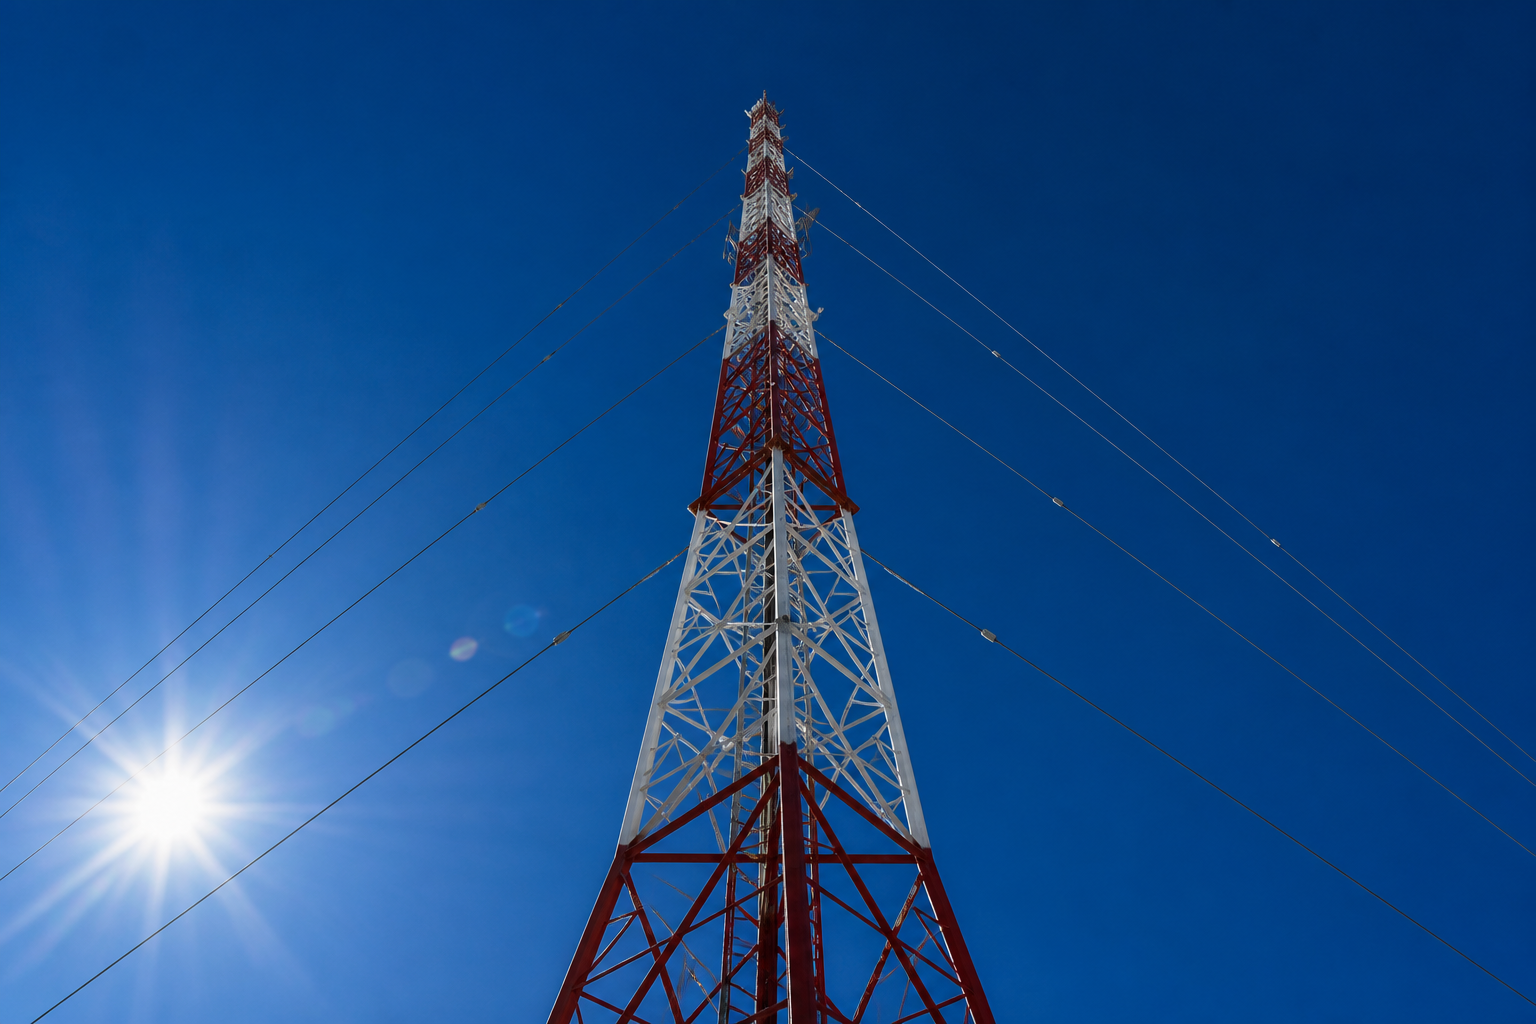
\includegraphics[width=0.54\linewidth]{images/book4/ai/b4-17-radio-mast-blue-sky.png}

{\small صارٍ للبثّ تحت سماء زرقاء: ثنائي قطب شاقولي بعلوّ عشرات الأمتار يشعّ نحو الأفق، وفوقه سماء تضيئها مليارات ثنائيات القطب الجزيئية وهي تعيد إشعاع الشمس.}
\end{omfigure}


\section{حقل ثنائي قطب متذبذب}

\begin{theorem}[حقل إشعاع ثنائي قطب كهربائي]\label{thm:b2:dipole-radiation:field}
\index{ثنائي قطب متذبذب}\index{منطقة الإشعاع}\index{تأخّر}
ثنائي قطب عزمه $\vect p(t) = p_0\cos\omega t\,\vect e_z$، وامتداده $a$، في
المبدأ، يشعّ. وفي \emph{\omterm{thm:b2:dipole-radiation:field}{منطقة الإشعاع}} --- أي على أبعاد $r \gg
\lambda = 2\pi c/\omega \gg a$ --- يكون حقله، في الإحداثيات الكروية $(r,
\theta, \varphi)$ حول محور ثنائي القطب، هو
\[
\vect E(M, t) = -\frac{\mu_0\,\omega^2p_0}{4\pi}\,\frac{\sin\theta}r\,\cos\bigl(\omega(t - r/c)\bigr)\,\vect e_\theta ,
\qquad
\vect B = \frac{\vect e_r\wedge\vect E}c :
\]
أي \omterm{prop:b2:sound-waves:spherical}{موجة كروية}، مستوية محليًّا --- إذ يؤلف $(\vect E, \vect B, \vect e_r)$
ثلاثيًّا مباشرًا مع $B = E/c$ --- \emph{متأخرة} بزمن الانتقال
$r/c$، وسعتها تتناقص وفق $1/r$، وهي متناسبة مع التسارع
$\ddot p = -\omega^2p$ لثنائي القطب ومع $\sin\theta$: فهي عظمى في
المستوي الاستوائي، ومنعدمة على المحور؛ ومستقطبة في المستوي
الذي يحوي المحور.
\end{theorem}
\admitted

\begin{remark}[قراءة الصيغة]\label{rem:b2:dipole-radiation:reading}
يحوي الحلّ المضبوط \omterm{thm:b2:maxwell-equations:maxwell}{لمعادلات ماكسويل} (انطلاقًا من الكمونات
المتأخرة، وهو خارج هذا المجلد) حدودًا في $1/r^2$ و
$1/r^3$ أيضًا؛ والأخير هو حقل ثنائي القطب شبه الساكن في مجلد
السنة الأولى، $\vect E \propto p/4\pi\varepsilon_0r^3$، وهو الغالب في \emph{المنطقة
القريبة} $r \ll \lambda$؛ وعند $r \sim \lambda/2\pi$ يتقارب الحدّان، وفي ما وراءها
لا يبقى إلا الحدّ $1/r$. ولكل عامل سببه. فأما $1/r$: فلأن
الاستطاعة عبر كرة، وهي $\propto E^2r^2$، يجب ألا تتعلق بالبعد $r$. وأما $\omega^2p_0$:
فلأن حقل شحنة ساكنة أو منتظمة الحركة ليس إشعاعيًّا؛ فالذي
يشعّ هو \emph{التسارع}. وأما $\sin\theta$: فالراصد على
المحور يرى الشحنة تذهب وتجيء على خط النظر، بلا تسارع
مستعرض؛ وفي المستوي الاستوائي يكون التسارع كله
مستعرضًا. وأما التأخّر: فالحقل عند $M$ في اللحظة $t$
يعكس ما فعله ثنائي القطب في $t - r/c$.
\end{remark}

\begin{omfigure}
\begin{tikzpicture}[font=\small, x=1cm, y=1cm, >=Stealth]
  \begin{scope}
    \draw[->, thick] (0,-2.2) -- (0,2.4) node[right, font=\footnotesize] {$z$};
    \draw[omThm, very thick, <->] (0,-0.5) -- (0,0.5); \node[omThm, font=\footnotesize] at (0.35,0.0) {$\vect p$};
    \coordinate (M) at (2.6,1.6);
    \draw[dashed] (0,0) -- (M); \fill (M) circle (1.5pt); \node[font=\footnotesize] at (2.45,1.25) {$M$};
    \draw (0,0.7) arc[start angle=90, end angle=31.6, radius=0.7]; \node[font=\footnotesize] at (0.35,0.9) {$\theta$};
    \draw[omDef, very thick, ->] (M) -- ($(M)+(0.55,-0.9)$) node[right, font=\footnotesize] {$\vect E$ ($\vect e_\theta$)};
    \node[omProp, font=\footnotesize] at ($(M)+(-0.65,0.25)$) {$\vect B$ $\otimes$};
    \draw[omExo, thick, ->] (M) -- ($(M)+(0.7,0.43)$) node[right, font=\footnotesize] {$\vect e_r$};
    \node[font=\footnotesize] at (0,-2.7) {$E \propto \dfrac{\omega^2p_0\sin\theta}{r}\cos\omega(t - r/c)$};
  \end{scope}
  \begin{scope}[xshift=8.6cm]
    \draw[->, thick] (0,-2.2) -- (0,2.4) node[right, font=\footnotesize] {$z$};
    \draw[omThm, thick, domain=0:360, samples=120, smooth] plot ({2.0*sin(\x)*sin(\x)*sin(\x)},{2.0*sin(\x)*sin(\x)*cos(\x)});
    \draw[omThm, very thick, <->] (0,-0.35) -- (0,0.35);
    \node[omThm, font=\footnotesize] at (2.3,0.35) {$\sin^2\theta$};
    \node[font=\footnotesize] at (0,-2.7) {الاستطاعة المشعّة في وحدة الزاوية المجسمة};
  \end{scope}
\end{tikzpicture}

{\small على اليسار: حقل إشعاع ثنائي قطب عند نقطة بعيدة $M$ ---
مستعرض، وفق $\vect e_\theta$، مع $\vect B$ سمتيّ؛ ولا يُشعّ شيء
على المحور. وعلى اليمين: \omterm{prop:b2:dipole-radiation:power}{نقش الإشعاع}، وهو كعكة
$\propto\sin^2\theta$ رُسم مقطعها.}
\end{omfigure}

\section{الاستطاعة المشعّة}

\begin{proposition}[استطاعة ثنائي قطب؛ صيغة لارمور]\label{prop:b2:dipole-radiation:power}
\index{استطاعة مشعّة (ثنائي قطب)}\index{صيغة لارمور}\index{نقش الإشعاع}
متوسط شعاع بوينتنغ لحقل ثنائي القطب قطريّ،
\[
\langle\vect\Pi\rangle = \frac{\mu_0\,\omega^4p_0^2}{32\pi^2c}\,\frac{\sin^2\theta}{r^2}\,\vect e_r ,
\]
ومتوسط الاستطاعة الكلية المشعّة هو
\[
\mathcal P = \frac{\mu_0\,\omega^4p_0^2}{12\pi c} = \frac{p_0^2\omega^4}{12\pi\varepsilon_0c^3} .
\]
ومن أجل شحنة وحيدة $q$ تسارعها $a$ (لانسبيًّا)، تكون
الاستطاعة اللحظية $\mathcal P = q^2a^2/6\pi\varepsilon_0c^3$ (لارمور).
\end{proposition}

\begin{proof}
$\langle\Pi\rangle = \langle E^2\rangle/\mu_0c$ مع $\langle\cos^2\rangle = \tfrac12$؛
وبالمكاملة على الكرة:
\[
\int\sin^2\theta\,r^2\dd\Omega = 2\pi r^2\int_0^\pi\sin^3\theta\,\dd\theta = \tfrac83\pi r^2 ,
\qquad
\mathcal P = \frac{\mu_0\omega^4p_0^2}{32\pi^2c}\cdot\frac{8\pi}3 = \frac{\mu_0\omega^4p_0^2}{12\pi c} .
\]
وأما لارمور: فيكون $p = qz$، ومن ثَمّ $\ddot p = qa$؛
واستبدال المتوسط $\tfrac12\omega^4p_0^2 = \langle\ddot p^2\rangle$ باللحظي
$q^2a^2$ يعطي $\mathcal P = \mu_0q^2a^2/6\pi c$.
\end{proof}

\begin{example}[هوائي وسلك]\label{ex:b2:dipole-radiation:antenna}
\index{هوائي}\index{مقاومة الإشعاع}\index{ثنائي قطب نصف موجي}
سلك قصير طوله $\ell \ll \lambda$ يحمل التيار $I_0\cos\omega t$ هو
ثنائي قطب عزمه $\dot p = I_0\ell\cos\omega t$، أي $p_0 = I_0\ell/\omega$: فيشعّ
$\mathcal P = \mu_0\omega^2I_0^2\ell^2/12\pi c = \tfrac12R_{\text{إشعاع}}I_0^2$ مع
\emph{\omterm{ex:b2:dipole-radiation:antenna}{مقاومة الإشعاع}} $R_{\text{إشعاع}} = \dfrac{2\pi}3\sqrt{\dfrac{\mu_0}{\varepsilon_0}}
\Bigl(\dfrac\ell\lambda\Bigr)^2 \approx 790\,(\ell/\lambda)^2\ \Omega$ --- فالاستطاعة تخرج من
الدارة كأنها تعبر مقاومة، من غير أن تسخّن شيئًا. وسلك طوله \qty{1}{m}
عند \qty{1}{MHz} ($\lambda = \qty{300}{m}$): $R_{\text{إشعاع}} = \qty{9}{m\ohm}$، أي أقلّ من
مقاومته النحاسية، وهو هوائي رديء؛ وعند \qty{100}{MHz}: \qty{88}{\ohm} (وصيغة
ثنائي القطب القصير مشدودة هنا)، وهو هوائي جيد. وأما \emph{\omterm{ex:b2:dipole-radiation:antenna}{ثنائي القطب
النصف موجي}}، $\ell = \lambda/2$ بتوزيع تيار جيبي، فله
$R_{\text{إشعاع}} = \qty{73}{\ohm}$ (وهو مقبول) ونقش قريب من نقش
ثنائي القطب الابتدائي --- وهو الهوائي القياسي، من صواري الراديو إلى
أذني الأرنب في التلفازات القديمة. وسلك شبكة طوله \qty{1}{m} عند \qty{50}{Hz}:
$R_{\text{إشعاع}} \approx \qty{2e-11}{\ohm}$ --- فالدارات شبه المستقرة في
\cref{ch:b2:maxwell-equations} لا تشعّ شيئًا.
\end{example}

\begin{omfigure}
\begin{tikzpicture}[font=\small, x=1cm, y=1cm, >=Stealth]
  \begin{scope}
    \draw[thick] (-2.4,0) -- (-0.15,0); \draw[thick] (0.15,0) -- (2.4,0);
    \draw[omExo, thick] (-0.15,0) -- (-0.15,-0.6) (0.15,0) -- (0.15,-0.6);
    \node[omExo, font=\footnotesize] at (0,-0.9) {التغذية};
    \draw[omThm, thick, domain=-2.4:2.4, samples=60] plot (\x,{1.0*cos(deg(pi*\x/4.8))});
    \foreach \x in {-2.0,-1.2,-0.4,0.4,1.2,2.0} \draw[omThm, ->] (\x,0) -- (\x,{1.0*cos(deg(pi*\x/4.8))});
    \node[omThm, font=\footnotesize] at (1.5,1.25) {$I(z)$};
    \draw[<->] (-2.4,-1.3) -- (2.4,-1.3) node[midway, below, font=\footnotesize] {$\lambda/2$};
    \node[font=\footnotesize] at (0,-2.2) {ثنائي قطب نصف موجي: $R_{\text{إشعاع}} = \qty{73}{\ohm}$};
  \end{scope}
  \begin{scope}[xshift=8.0cm]
    \begin{axis}[omaxis, axis x line=bottom, axis y line=left, width=5.6cm, height=4.2cm, at={(0,-1.9cm)},
        xmode=log, ymode=log, xmin=1e-3, xmax=0.5, ymin=1e-3, ymax=300,
        xlabel={$\ell/\lambda$}, ylabel={$R_{\text{إشعاع}}$ ($\Omega$)}, xtick={1e-3,1e-2,1e-1}, ytick={1e-3,1e-1,10},
        xlabel style={at={(axis description cs:0.5,-0.12)}, anchor=north},
        ylabel style={at={(axis description cs:-0.2,0.5)}, rotate=90, anchor=south}, samples=40]
      \addplot[omDef, thick, domain=1e-3:0.3] {790*x*x};
      \addplot[only marks, mark=*, mark size=1.8pt, omThm] coordinates {(0.5,73)};
    \end{axis}
  \end{scope}
\end{tikzpicture}

{\small على اليسار: توزيع التيار على \omterm{ex:b2:dipole-radiation:antenna}{ثنائي قطب نصف موجي}، وهو أعظم
عند التغذية ومنعدم عند الطرفين. وعلى اليمين: مقاومة إشعاع
ثنائي قطب قصير، $790(\ell/\lambda)^2$ أوم، و \qty{73}{\ohm} \omterm{ex:b2:dipole-radiation:antenna}{لثنائي القطب
النصف موجي}.}
\end{omfigure}

\begin{example}[إلكترون يشعّ]\label{ex:b2:dipole-radiation:electron}
في أنبوب أشعة سينية يتوقف إلكترون طاقته \qty{50}{keV} ($v = \qty{1.2e8}{m/s}$)
في \qty{1}{\micro m} من التنغستن: $a \sim v^2/2d = \qty{7e21}{m/s^2}$، واستطاعة لارمور
$\qty{1.2e-4}{W}$ خلال $\qty{1.6e-14}{s}$: أي \qty{2e-18}{J}، ونحو $0.02\%$ من
طاقته يُشعّ إشعاعَ الكبح (بريمشترالونغ) في
الأنبوب --- والباقي حرارة، ولذلك يُبرَّد المصعد. وأما إلكترون
ذرة الهدروجين الكلاسيكي، وتسارعه $v^2/r = \qty{9e22}{m/s^2}$،
فكان يشعّ \qty{5e-8}{W} ويهوي حلزونيًّا إلى النواة في \qty{1e-11}{s}:
فالفيزياء الكلاسيكية تمنع الذرات، و\cref{ch:b2:schrodinger-wave-functions}
ينقذها.
\end{example}

\section{تبعثر رايلي: السماء الزرقاء}

\begin{proposition}[التبعثر على إلكترون مرتبط]\label{prop:b2:dipole-radiation:rayleigh}
\index{تبعثر رايلي}\index{مقطع عرضي للتبعثر}\index{تبعثر طومسون}
موجة سعتها $E_0$ وتواترها $\omega$ ترد على ذرة تُنمذَج
إلكترونًا مرتبطًا ارتباطًا مرنًا رنينه $\omega_0 \gg \omega$
(\cref{ch:b2:waves-in-media}): فيتذبذب الإلكترون بسعة
$eE_0/m\omega_0^2$، وتصير الذرة ثنائي قطب $p_0 = e^2E_0/m\omega_0^2$ موافقًا في الطور
للحقل، وتعيد إشعاع الاستطاعة $\mathcal P = p_0^2\omega^4/12\pi
\varepsilon_0c^3$. ونسبة تلك الاستطاعة إلى الشدة الواردة هي
\emph{\omterm{prop:b2:dipole-radiation:rayleigh}{المقطع العرضي للتبعثر}}
\[
\sigma = \frac{\mathcal P}{\varepsilon_0cE_0^2/2} = \frac{8\pi}3\,r_e^2\Bigl(\frac\omega{\omega_0}\Bigr)^4 ,
\qquad r_e = \frac{e^2}{4\pi\varepsilon_0mc^2} = \qty{2.8e-15}{m} :
\]
أي قانون رايلي، $\sigma \propto \omega^4 \propto 1/\lambda^4$. وأما الإلكترون \emph{الحر}
($\omega_0 = 0$) فمقطعه العرضي $\sigma_T = 8\pi r_e^2/3 =
\qty{6.65e-29}{m^2}$، ولا يتعلق بالتواتر (\omterm{prop:b2:dipole-radiation:rayleigh}{تبعثر طومسون}).
\end{proposition}

\begin{proof}
من نموذج لورنتز مع $\omega \ll \omega_0$ وتخامد مهمَل،
$\underline{\vect r} = -e\underline{\vect E}/m\omega_0^2$؛ عوّض $p_0$ في الاستطاعة
واقسم على $I = \varepsilon_0cE_0^2/2$؛ و $r_e$ يجمع الثوابت. وأما الإلكترون
الحر: $\vect r = e\vect E/m\omega^2$ (في تعاكس الطور)، و $p_0 = e^2E_0/m\omega^2$، فيختصر
$\omega^4$.
\end{proof}

\begin{example}[سماء زرقاء، وغروب أحمر، وغيوم بيضاء]\label{ex:b2:dipole-radiation:sky}
الضوء البنفسجي ($\qty{400}{nm}$) يتبعثر $(700/400)^4 = 9.4$ ضعف ما يتبعثر
الأحمر: فالسماء، وهي مضاءة بضوء الشمس المتبعثر، زرقاء (لا بنفسجية:
إذ تصدر الشمس بنفسجيًّا أقلّ وتراه العين رؤية سيئة). وعند الغروب يقطع
الضوء المباشر من الهواء أربعين ضعف ما يقطعه عند الظهر ويفقد زرقته
لسماء أماكن أخرى: فيحمرّ. وكل جزيء هواء يتبعثر بمقطع
$\sigma \approx \qty{5e-31}{m^2}$ عند \qty{550}{nm}؛ ومع $n = \qty{2.5e25}{m^{-3}}$ يكون
المسار الحر الوسطي $1/n\sigma$ هو \qty{80}{km}: أي إن عُشر الضوء الأخضر
يتبعثر في نزوله عبر الجوّ، وثلث
البنفسجي. وأما قطيرات الغيوم، وهي أكبر بكثير من $\lambda$، فليست
مبعثرات رايلي: إذ تبعثر الألوان كلها بالسواء --- فتكون بيضاء.
\end{example}

\begin{proposition}[الاستقطاب بالتبعثر]\label{prop:b2:dipole-radiation:polarization}
\index{استقطاب بالتبعثر}
\omterm{def:b2:plane-waves-polarization:states}{الضوء الطبيعي} المنتشر وفق $x$ يحدث ثنائيات قطب في المستوي $yz$.
والراصد الناظر وفق $y$ (أي على \qty{90}{\degree} من الحزمة) لا يتلقى
إشعاعًا من مركّبات ثنائي القطب وفق $y$ (وهي خط نظره)
ويتلقى الإشعاع كله من المركّبات وفق $z$: فالضوء المتبعثر
\emph{مستقطب خطيًّا} وفق $z$، عموديًّا على المستوي
الذي يحوي الحزمة وخط النظر. وعند الزوايا الأخرى يكون
مستقطبًا جزئيًّا، بالدرجة $(1 - \cos^2\chi)/(1 + \cos^2\chi)$ من أجل
زاوية التبعثر $\chi$.
\end{proposition}

\begin{proof}
\omterm{def:b2:plane-waves-polarization:states}{للضوء الطبيعي} الوارد $\vect E$ ذو مركّبتين متوسطاهما متساويان
وفق $y$ و $z$؛ وثنائي القطب وفق $y$ لا يشعّ نحو $y$ ($\sin
\theta = 0$)، وأما الذي وفق $z$ فيشعّ $\propto\sin\theta = 1$. وعند الزاوية $\chi$
تنقص مساهمة المركّبة $y$ بالعامل $\cos^2\chi$ في الشدة.
\end{proof}

\begin{omfigure}
\begin{tikzpicture}[font=\small, x=1cm, y=1cm, >=Stealth]
  \draw[omDef, very thick, ->] (-4.4,0) -- (-0.4,0) node[above, pos=0.3, font=\footnotesize] {ضوء الشمس (طبيعي)};
  \draw[omDef, thick, <->] (-1.3,-0.45) -- (-1.3,0.45); \node[omDef, font=\footnotesize] at (-0.95,-0.45) {$\vect E_z$};
  \node[omDef, font=\footnotesize] at (-2.6,-0.4) {$\vect E_y$ $\odot$};
  \fill[omExo] (0,0) circle (3pt); \node[font=\footnotesize] at (0.1,-0.45) {جزيء};
  \draw[omThm, very thick, ->] (0.3,0.3) -- (2.6,2.6) node[right, font=\footnotesize] {إلى الأمام: غير مستقطب};
  \draw[omThm, very thick, ->] (0,0.45) -- (0,3.0) node[above, font=\footnotesize] {\qty{90}{\degree}: مستقطب $\perp$ المستوي};
  \node[omThm, font=\footnotesize] at (0.75,2.3) {$\odot$ فقط};
  \draw[omThm, very thick, ->] (0.45,0) -- (3.6,0) node[right, font=\footnotesize] {غير مستقطب};
\end{tikzpicture}

{\small ضوء الشمس متبعثرًا على جزيء هواء: لثنائي القطب المحدَث
مركّبات عمودية على الحزمة؛ والراصد على \qty{90}{\degree}
لا يتلقى إلا المركّبة العمودية على خط نظره ---
أي ضوءًا مستقطبًا خطيًّا. والسماء هناك أشدّ زرقة وأشدّ استقطابًا.}
\end{omfigure}

\begin{remark}[لمَ يبلغنا الضوء الأزرق أصلًا]\label{rem:b2:dipole-radiation:why}
في وسط منتظم تمامًا تتداخل الأمواج المتبعثرة على الجزيئات
المتجاورة تداخلًا هدّامًا في كل جهة إلا الأمامية
(وقرينة الانكسار هي تلك الموجة المتبعثرة أمامًا). والذي
يترك شدة متبعثرة صافية هو \emph{تقلّبات} كثافة الهواء --- إذ
ليست الجزيئات على شبكة --- وهي متناسبة مع
عدد الجزيئات، كما حُسب أعلاه من أجل واحد (أينشتاين، 1910). وهذا
العشوائي نفسه يجعل ضوء السماء غير مترابط من نقطة إلى أخرى.
\end{remark}

\begin{method}[تقديرات الإشعاع]\label{met:b2:dipole-radiation:method}
(1) عيّن ثنائي القطب: $p_0 = q\,\times$ السعة، أو $I_0\ell/\omega$ من أجل
سلك. (2) والحقل على البعد $r$: $E \approx \mu_0\omega^2p_0\sin\theta/4\pi r$؛ والاستطاعة:
$\mu_0\omega^4p_0^2/12\pi c$. (3) ومن أجل شحنة متسارعة استعمل لارمور؛ ومن أجل
هوائي استعمل \omterm{ex:b2:dipole-radiation:antenna}{مقاومة الإشعاع}. (4) وفي التبعثر، احسب ثنائي القطب
المحدَث من استجابة الوسط (بنموذج لورنتز) واقسم
الاستطاعة المشعّة على الشدة الواردة. (5) وتذكّر الأصفار:
فلا شيء على محور التذبذب، ومن هنا الاستقطاب عند
\qty{90}{\degree} \omterm{prop:b2:wave-interfaces:brewster}{وزاوية بروستر} في \cref{ch:b2:wave-interfaces}.
\end{method}

\section{تمارين}

\begin{exercise}[$\star$]\label{exo:b2:dipole-radiation:1}
هوائي قصير طوله \qty{1.0}{m} يحمل \qty{2.0}{A} (سعةً) عند
\qty{100}{MHz}. أوجد سعة ثنائي القطب $p_0$؛ وسعة الحقل على \qty{1}{km} في
المستوي الاستوائي وعلى \qty{30}{\degree} من المحور؛ والاستطاعة المشعّة؛
\omterm{ex:b2:dipole-radiation:antenna}{ومقاومة الإشعاع}.
\end{exercise}

\begin{exercise}[$\star$]\label{exo:b2:dipole-radiation:2}
أوجد مقاومة إشعاع سلك طوله \qty{1}{m} عند \qty{100}{kHz}، و \qty{1}{MHz}،
و \qty{10}{MHz}، و \qty{100}{MHz}؛ وقارنها بمقاومته النحاسية
(قطره \qty{1}{mm}، مع \omterm{thm:b2:waves-in-media:skin}{الأثر القشري} عند التواترات العليا،
$\delta = \qty{0.2}{mm}$ عند \qty{100}{kHz})؛ وأوجد المردود (المشعّ على الكلي)
في كل حالة. ولمَ تكون صواري مرسلات الموجة الطويلة بعلوّ مئات
الأمتار؟
\end{exercise}

\begin{exercise}[$\star$]\label{exo:b2:dipole-radiation:3}
أوجد نسبة \omterm{prop:b2:dipole-radiation:rayleigh}{تبعثر رايلي} للضوء عند \qty{400}{nm}، و \qty{550}{nm}، و
\qty{700}{nm}؛ ولطولي موجة الرادار \qty{3}{cm} و \qty{10}{cm} على
قطرات المطر (لو كانت صغيرة كفاية --- وهي ليست كذلك تمامًا)؛ ولمَ
يستعمل رادار الطقس أطوال موجة قصيرة ليرى المطر وطويلة ليرى
عبره؟
\end{exercise}

\begin{exercise}[$\star$]\label{exo:b2:dipole-radiation:4}
أوجد درجة استقطاب ضوء السماء على \qty{30}{\degree}، و \qty{60}{\degree}،
و \qty{90}{\degree}، و \qty{120}{\degree} من الشمس؛ وإلى أين في السماء يوجّه
المصوّر مستقطبًا ليحصل على أشدّ زرقة داكنة، وماذا
يحدث حين تكون الشمس في السمت؟ ولمَ لا يتجاوز العظم الحقيقي
$75\%$ (فكّر في التبعثر المتعدد وفي ما تعكسه الأرض)؟
\end{exercise}

\begin{exercise}[$\star\star$]\label{exo:b2:dipole-radiation:5}
(أ) كامِل شعاع بوينتنغ لثنائي القطب على كرة
وتحقق من $\mathcal P = \mu_0\omega^4p_0^2/12\pi c$. (ب) وأوجد النسبة من الاستطاعة
المشعّة ضمن \qty{30}{\degree} من المستوي الاستوائي. (ج) وزاوية نصف
الاستطاعة: عند أي $\theta$ تكون الشدة نصف عظمها؟ (د) و"مكسب"
ثنائي القطب، أي عظم الشدة على المتوسط المتماثل المناحي:
بيّن أنه $1.5$.
\end{exercise}

\begin{exercise}[$\star\star$]\label{exo:b2:dipole-radiation:6}
\emph{القريب والبعيد.} (أ) اكتب حقل ثنائي القطب شبه الساكن عند
$\theta = 90^\circ$، $E_{\text{قريب}} = p/4\pi\varepsilon_0r^3$، والحقل الإشعاعي؛ وعلى
أي بعد $r_0$ تتساوى سعتاهما؟ وعبّر عن $r_0$ بدلالة
$\lambda$. (ب) ومن أجل هوائي عند \qty{1}{MHz}، أوجد $r_0$؛ وأيّ الحقلين يحسّه مستقبل
على \qty{10}{m}، وأيّهما على \qty{10}{km}؟ (ج) وهاتف محمول عند \qty{1}{GHz} يُمسَك
على \qty{2}{cm} من الرأس: أفي المنطقة القريبة هو أم البعيدة؟ (د) ولمَ لا يحمل الحقل
القريب استطاعة صافية بعيدًا؟
\end{exercise}

\begin{exercise}[$\star\star$]\label{exo:b2:dipole-radiation:7}
\emph{طومسون والإكليل.} (أ) احسب $\sigma_T$. (ب) وفي إكليل الشمس
$n_e \approx \qty{1e14}{m^{-3}}$ على $10^9$ متر: أوجد النسبة من ضوء الكرة الضوئية
المتبعثر نحونا؛ ولمَ يكون الإكليل أبيض ولا يُرى إلا
في أثناء الكسوف؟ (ج) وأشعة سينية طاقتها \qty{10}{keV} على ذرة كربون ($6$
إلكترونات، وطاقات ارتباطها دون \qty{300}{eV}): لمَ تتبعثر الإلكترونات
كأنها حرة، وما مقطع الذرة العرضي؟ (د) ولمَ
تختلف صورة العظم بالأشعة السينية عن اللحم بالامتصاص أساسًا،
لا \omterm{prop:b2:dipole-radiation:rayleigh}{بتبعثر طومسون}؟
\end{exercise}

\begin{exercise}[$\star\star$]\label{exo:b2:dipole-radiation:8}
\emph{الغروب.} العمق البصري للجوّ من أجل \omterm{prop:b2:dipole-radiation:rayleigh}{تبعثر
رايلي} في السمت هو $\tau(\lambda) = 0.1\,(550\,\text{nm}/\lambda)^4$ (ويُوهَن
الضوء المباشر بالعامل $\eu^{-\tau}$). (أ) أوجد النفاذية في
السمت عند \qty{400}{nm}، و \qty{550}{nm}، و \qty{700}{nm}. (ب) وعند الغروب يطول المسار
$38$ ضعفًا: أوجد النفاذيات؛ ونسبة الأحمر إلى الأزرق. (ج) ولمَ
يحمرّ القمر في أثناء خسوفه؟ (د) ولمَ تكون السماء قرب
الأفق بيضاء لا زرقاء غامقة؟
\end{exercise}

\begin{exercise}[$\star\star$]\label{exo:b2:dipole-radiation:9}
\emph{هوائيان.} ثنائيا قطب شاقوليان يبعد أحدهما عن الآخر $d$ وفق
$x$ يُغذَّيان بالسعة نفسها. (أ) على توافق الطور، $d = \lambda/2$: في أي
الجهات الأفقية يتجمع حقلاهما البعيدان، وفي أيها يتلاشيان؟
(وهي الرصّة العرضية). (ب) وعلى تعاكس الطور، $d = \lambda/2$: الشيء نفسه (الرصّة الطرفية).
(ج) وعلى التربيع، $d = \lambda/4$: بيّن أن الرصّة تشعّ نحو جهة
واحدة فقط. (د) ولمَ تستعمل محطات البثّ AM عدة صوارٍ، وكيف
يوجّه رادار الرصّة الطورية حزمته من غير حركة؟
\end{exercise}

\begin{exercise}[$\star\star\star$]\label{exo:b2:dipole-radiation:10}
\emph{التخامد الإشعاعي.} إلكترون لورنتز (\cref{ch:b2:waves-in-media})
المتذبذب عند $\omega_0$ بسعة $x_0$ يشعّ بصيغة لارمور.
(أ) أوجد متوسط الاستطاعة المشعّة؛ وطاقة المذبذب $\tfrac12m\omega_0^2x_0^2$؛
وبيّن أن الطاقة تتناقص بالمعدل $\Gamma = e^2\omega_0^2/6\pi\varepsilon_0mc^3$.
(ب) وأوجد قيمة $\Gamma$ من أجل خط الصوديوم (\qty{589}{nm})؛ وقارنها بالمقدار
$\Gamma$ المستعمل في \cref{exo:b2:waves-in-media:9}. (ج) والعمر $1/\Gamma$ والعرض
الطبيعي للخط، $\Delta\lambda = \lambda^2\Gamma/2\pi c$. (د) وعامل جودة
المذبذب الذري $\omega_0/\Gamma$.
\end{exercise}

\begin{exercise}[$\star\star\star$]\label{exo:b2:dipole-radiation:11}
\emph{الصاري.} محطة AM تشعّ \qty{50}{kW} عند \qty{1}{MHz} من
صارٍ شاقولي ارتفاعه $\lambda/4$ على أرض ناقلة (وهي تعمل
مرآةً، فتجعل الصاري نصف \omterm{ex:b2:dipole-radiation:antenna}{ثنائي قطب نصف موجي}: $R_{\text{إشعاع}} \approx
\qty{36}{\ohm}$، وتذهب الاستطاعة إلى نصف الفضاء العلوي وحده). (أ)
أوجد الارتفاع؛ والتيار عند القاعدة. (ب) وسعة الحقل على \qty{10}{km} في
المستوي الأفقي (استعمل نقش ثنائي القطب، و $\mathcal P$ على نصف الكرة
العلوي $= \int\langle\Pi\rangle\dd S$؛ وخذ $\langle\Pi\rangle = 1.5\,
\mathcal P/2\pi r^2$ عند الأفق تقديرًا معقولًا). (ج) والقوة المحركة في
سوط استقبال طوله \qty{1}{m} هناك. (د) ولمَ تهمّ ناقلية الأرض،
ولمَ تُدفن أسلاك نحاسية قطرية تحت الصاري؟
\end{exercise}

\begin{exercise}[$\star\star\star$]\label{exo:b2:dipole-radiation:12}
\emph{التبعثر والقرينة.} في غاز مخلخل تتجمع الأمواج المتبعثرة
أمامًا على الجزيئات كلها تجمعًا مترابطًا فتبني قرينة الانكسار،
$n - 1 = N\alpha/2\varepsilon_0$ حيث $\alpha = e^2/m\omega_0^2$ هي الاستقطابية؛ ومقطع
رايلي العرضي هو $\sigma = (8\pi/3)r_e^2(\omega/\omega_0)^4$. (أ) عبّر عن
$\sigma$ بدلالة $n$ و $N$ و $\lambda$: $\sigma = 8\pi^3(n^2 - 1)^2/3N^2\lambda^4$. (ب)
ومن أجل الهواء ($n - 1 = 2.9 \times 10^{-4}$، و $N = \qty{2.5e25}{m^{-3}}$) عند \qty{550}{nm}:
أوجد $\sigma$ والمسار الحر الوسطي $1/N\sigma$. (ج) والعمق البصري الشاقولي
للجوّ (بارتفاع مكافئ \qty{8}{km})؛ وقارنه بالقيمة $0.1$ في
\cref{exo:b2:dipole-radiation:8}. (د) ولمَ أعطت هذه العلاقة (رايلي،
1899) قيمةً لعدد أفوغادرو؟
\end{exercise}

\section{مسألة: الصاري والسماء والإلكترون}

\begin{problem}[{مسألة نهاية الأسبوع --- ثلاثة هوائيات: صاري
بثّ، وجزيء هواء في ضوء الشمس، وإلكترون حر}]
\label{pb:b2:dipole-radiation:1}

\medskip
\noindent\textbf{الجزء الأول --- الصاري.}
محطة موجة متوسطة عند $f = \qty{1.0}{MHz}$ تشعّ $\mathcal P = \qty{100}{kW}$
من صارٍ ربع موجي على أرض ناقلة ($R_{\text{إشعاع}} = \qty{36}{\ohm}$،
ونقشه نقش ثنائي قطب شاقولي على نصف الفضاء العلوي، كما في
\cref{exo:b2:dipole-radiation:11}).
\begin{enumerate}
  \item أوجد طول الموجة وارتفاع الصاري؛ وسعة التيار عند
        قاعدته؛ والتوتر على $R_{\text{إشعاع}}$.
  \item وسعة عزم ثنائي القطب المكافئ، بمعاملة الصاري
        ثنائيَ قطب قصير $p_0 = I_0\ell_{\text{فعّال}}/\omega$، مع $\ell_{\text{فعّال}} \approx
        \lambda/2\pi$ من أجل الصاري الربع موجي (وهو مقبول).
  \item ومتوسط الشدة على \qty{10}{km} وعلى \qty{100}{km} في المستوي
        الأفقي (خذ نقش نصف الكرة العلوي، وهو أعظم عند
        الأفق، $\langle\Pi\rangle = 1.5\mathcal P/2\pi r^2$)؛ وسعتي الحقل.
  \item والقوة المحركة في سوط شاقولي طوله \qty{1}{m} على \qty{100}{km}؛ وفي
        هوائي قضيب فرّيتي (وشيعة من $N = 100$ لفة، \qty{1}{cm^2}،
        ونفوذية فعّالة $100$) مواجهًا حقلَ $\vect B$ للموجة: قارن.
  \item والاستطاعة التي يتلقاها مستقبِل موائم هوائيه
        مساحته الفعّالة $A = 1.5\lambda^2/4\pi$ (وهي مساحة ثنائي القطب) على \qty{100}{km}.
  \item ولنواقل الصاري مقاومة ضياع كلية
        \qty{2}{\ohm}: أوجد المردود؛ والاستطاعة الضائعة حرارةً.
  \item أيقع مستقبل على \qty{10}{km} في \omterm{thm:b2:dipole-radiation:field}{منطقة الإشعاع}؟ وآخر على
        \qty{100}{m} من الصاري؟
  \item ولمَ تبلغ إشارات الموجة المتوسطة أبعدَ ليلًا؟ (تذكّر
        الطبقة D في \cref{ch:b2:waves-in-media}.)
\end{enumerate}

\medskip
\noindent\textbf{الجزء الثاني --- السماء.}
الهواء عند مستوى البحر: $N = \qty{2.5e25}{m^{-3}}$، ومقطع رايلي العرضي $\sigma =
\qty{4.6e-31}{m^2}\,(550\,\text{nm}/\lambda)^4$؛ وضوء الشمس \qty{1.0}{kW/m^2} عند
الأرض؛ وسماكة الجوّ المكافئة عند كثافة مستوى البحر هي
\qty{8}{km}.
\begin{enumerate}[resume]
  \item أوجد المقطع العرضي عند \qty{450}{nm} وعند \qty{650}{nm}؛ والنسبة.
  \item والمسار الحر الوسطي للألوان الثلاثة؛ والعمق البصري الشاقولي
        $\tau = N\sigma H$؛ والنسبة المتبعثرة من كل لون خارج
        الحزمة المباشرة في السمت.
  \item والاستطاعة المتبعثرة في المتر المكعب من الهواء عند الأرض على
        الضوء الأخضر (خذ \qty{300}{W/m^2} من ضوء الشمس حول
        \qty{550}{nm})؛ وفي أي زاوية مجسمة، وبأي نقش؟
  \item وعمود هواء مقطعه \qty{1}{m^2} يُنظر إليه على \qty{90}{\degree} من
        الشمس: قدّر شدة ضوء السماء الواصل إلى
        الراصد من ذلك العمود (أي الاستطاعة المتبعثرة نحوه في
        وحدة الزاوية المجسمة، على امتداد \qty{8}{km})، وقارنها
        بالشمس المباشرة؛ أتكون سطوع السماء من الرتبة الصحيحة
        (نحو \qty{1e-5}{} من سطوع الشمس)؟
  \item ودرجة استقطاب الضوء الآتي من ذلك العمود؛ ولمَ تكون
        أدنى في الواقع، وكيف تستعملها بعض الحشرات؟
  \item وعند الغروب يكون المسار $38$ جوًّا: أوجد النسبتين النافذتين
        من الأزرق والأحمر؛ ولون الشمس؛ ولمَ تبقى السماء فوق الرأس
        زرقاء.
  \item ولمَ تكون السماء سوداء على القمر حتى في وضح النهار؟
  \item وعلى المريخ يكون الهواء أرقّ بمئة مرة لكنه مليء بغبار
        ناعم (حبيبات بالميكرومتر): لمَ تكون سماء المريخ
        بلون الكرمل وغروبها أزرق؟
\end{enumerate}

\medskip
\noindent\textbf{الجزء الثالث --- الإلكترون.}
\begin{enumerate}[resume]
  \item أوجد مقطع طومسون العرضي من $r_e$.
  \item وفي أنبوب أشعة سينية يتوقف إلكترون طاقته \qty{100}{keV} ($v = \qty{1.6e8}{m/s}$،
        عامله معاملة لانسبية) على \qty{2}{\micro m} في
        التنغستن: أوجد التسارع، واستطاعة لارمور، والمدة، والطاقة
        المشعّة ونسبتها من الطاقة الحركية.
  \item وأقصر طول موجة يستطيع الأنبوب إصداره (أي فوتون يأخذ
        طاقة الإلكترون كلها).
  \item ويعمل الأنبوب على \qty{20}{mA}: أوجد الاستطاعة المشعّة؛ والحرارة في المصعد؛
        ولمَ يدور المصعد.
  \item وإلكترون كلاسيكي يدور حول بروتون على نصف قطر بور
        (\qty{5.3e-11}{m}، بسرعة \qty{2.2e6}{m/s}): أوجد التسارع، واستطاعة
        لارمور، والزمن اللازم لإشعاع طاقته \qty{13.6}{eV} --- أي
        عمر الذرة الكلاسيكية.
  \item والذرات الحقيقية تدوم أبدًا: سمِّ ما تفوته الفيزياء الكلاسيكية
        هنا، وما ستقوله \cref{ch:b2:schrodinger-wave-functions}
        عن الحالة المستقرة.
  \item وإلكترون في سنكروترون نصف قطره \qty{100}{m} عند $v \approx c$:
        أيّ استطاعة تعطي صيغة لارمور اللانسبية؟ (والاستطاعة
        الحقيقية أكبر بالعامل $\gamma^4$، مع $\gamma \sim 10^4$: وهو
        منبع الضوء السنكروتروني.)
  \item والإلكترون نفسه ساكنًا في \qty{1}{kW/m^2} من ضوء الشمس:
        أوجد الاستطاعة التي يعيد إشعاعها (بطومسون)؛ وعدد الإلكترونات
        اللازم لتبعثر واط واحد.
  \item ولخّص الهوائيات الثلاثة في جدول: عزم ثنائي القطب،
        والتواتر، والاستطاعة، والنقش.
\end{enumerate}
\end{problem}
